\section{Experiment}

\begin{frame}{Experiment}

Goal: test if DISHTINY scheme selects for higher-order individuality

\end{frame}

\begin{frame}{What's Evolving?}

Manually-designed strategy parameters:
\begin{itemize}
\item Should I reproduce over a neighbor that shares my signaling channel?
\item Should I share resources with my signaling channel network?
\item How big should my signaling channel get before I start making propagules?
\item How much resource should I endow propagules with?
\item Should I attempt an apoptosis response to mutation?
\end{itemize}
\end{frame}

\section{Preliminary Results}
\section{Preliminary\** Results}


\begin{frame}{Outcomes}

Categorized outcomes by resource-sharing of dominant genotype:
\begin{itemize}
\item hog resources to cell
\begin{itemize}
\item cell-level individuals
\item \textit{rare outcome}
\end{itemize}
\item share resources with Level 1 same-channel network
\begin{itemize}
\item level-one individuals
\item \textit{frequent outcome}
\end{itemize}
\item share resources with Level 2 same-channel network
\begin{itemize}
\item level-two individuals
\item \textit{frequent outcome}
\end{itemize}
\end{itemize}

\end{frame}

\begin{frame}{Outcome: Cell-level Individuality}
\begin{figure}
\begin{columns}
\begin{column}{0.6\textwidth}
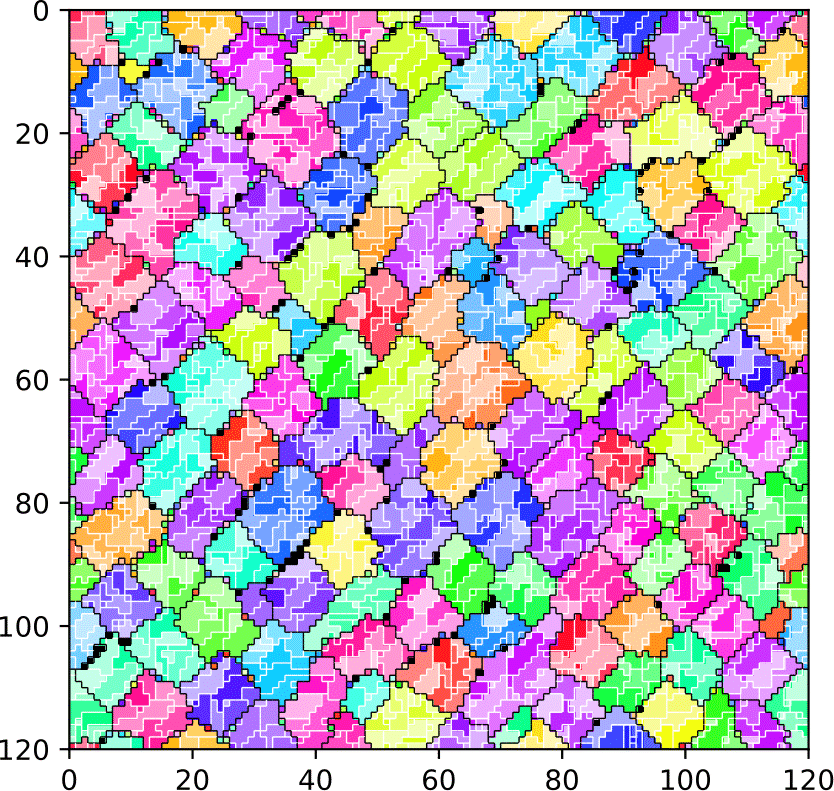
\includegraphics[width=\textwidth]{img/results/ChannelMap_1022_update19500000.png}
\end{column}
\begin{column}{0.4\textwidth}
\caption{
End state of same-channel signaling networks in simulation where cell-level individuality dominated.
}
\end{column}
\end{columns}
\end{figure}
\end{frame}

\begin{frame}{Outcome: Level-one Individuality}
\begin{figure}
\begin{columns}
\begin{column}{0.6\textwidth}
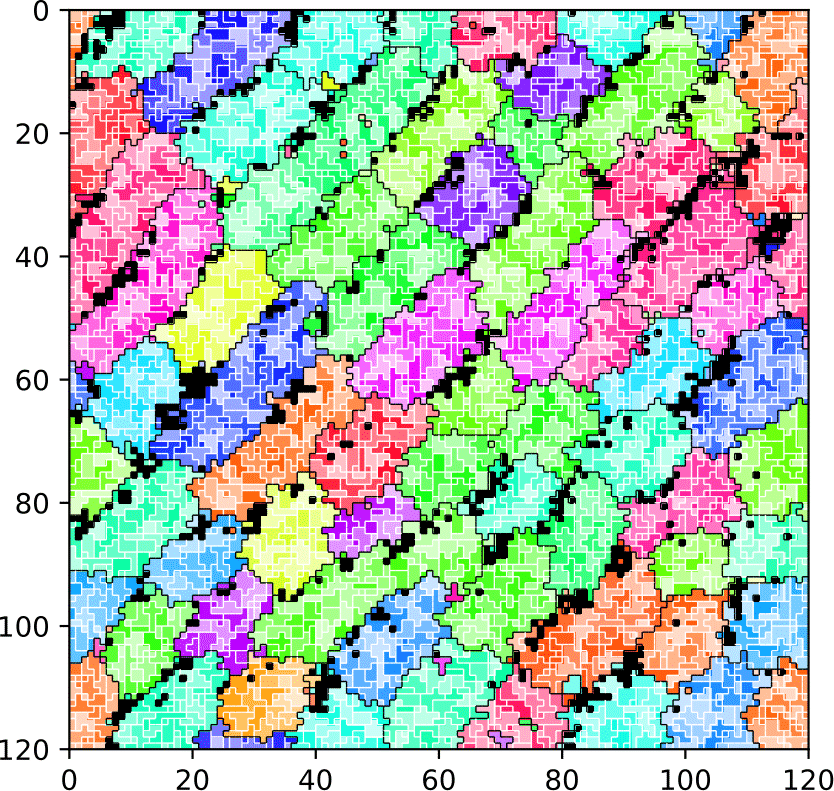
\includegraphics[width=\textwidth]{img/results/ChannelMap_1041_update19500000.png}
\end{column}
\begin{column}{0.4\textwidth}
\caption{
End state of same-channel signaling networks in simulation where level-one individuality dominated.
}
\end{column}
\end{columns}
\end{figure}
\end{frame}

\begin{frame}{Outcome: Level-two Individuality}
\begin{figure}
\begin{columns}
\begin{column}{0.6\textwidth}
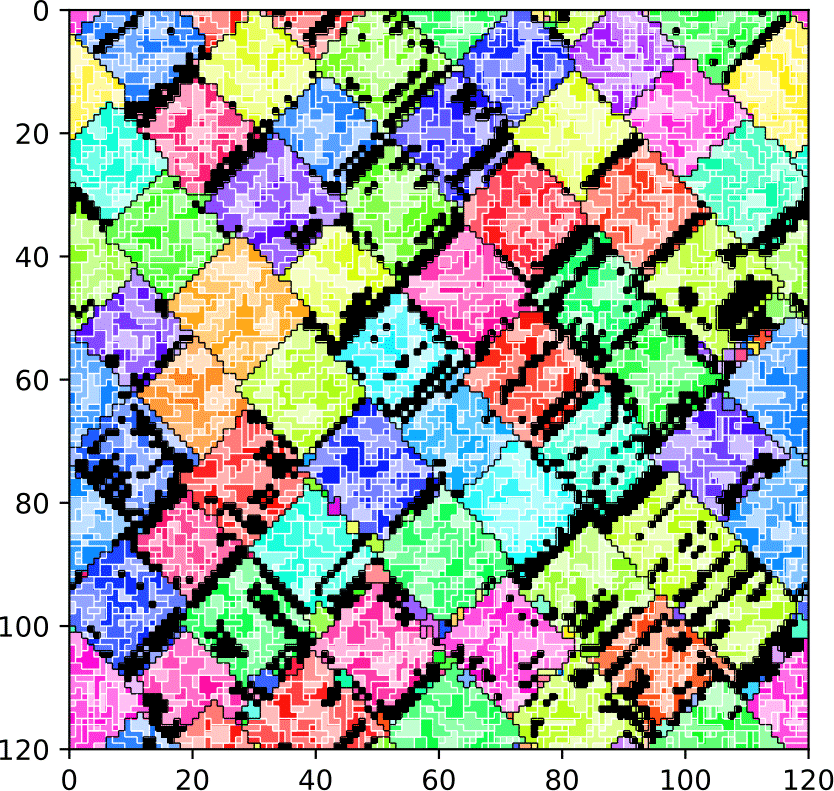
\includegraphics[width=\textwidth]{img/results/ChannelMap_1047_update19500000.png}
\end{column}
\begin{column}{0.4\textwidth}
\caption{
End state of same-channel signaling networks in simulation where level-two individuality dominated.
}
\end{column}
\end{columns}
\end{figure}
\end{frame}

\begin{frame}{Outcome: Evolution of Level-two Individuality}
\begin{figure}
\begin{columns}
\begin{column}{0.6\textwidth}
\includegraphics<1>[width=\textwidth]{results/ChannelMap_1011_update0.png}%
\includegraphics<2>[width=\textwidth]{results/ChannelMap_1011_update500000.png}%
\includegraphics<3>[width=\textwidth]{results/ChannelMap_1011_update1000000.png}%
\includegraphics<4>[width=\textwidth]{results/ChannelMap_1011_update2000000.png}%
\includegraphics<5>[width=\textwidth]{results/ChannelMap_1011_update4000000.png}%
\includegraphics<6>[width=\textwidth]{results/ChannelMap_1011_update5000000.png}%
\includegraphics<7>[width=\textwidth]{results/ChannelMap_1011_update7000000.png}%
\end{column}
\begin{column}{0.4\textwidth}
\only<1>{Update: 0}%
\only<2>{Update: 500,000}%
\only<3>{Update: 1,000,000}%
\only<4>{Update: 2,000,000}%
\only<5>{Update: 4,000,000}%
\only<6>{Update: 5,000,000}%
\only<7>{Update: 7,000,000}%

\vspace{8ex}

\caption{Channel-map visualization of a simulation where second-level individuality evolved.}
\end{column}
\end{columns}
\end{figure}
\end{frame}

\begin{frame}{Level-one vs. Level-two Relative Fitness}

\begin{figure}
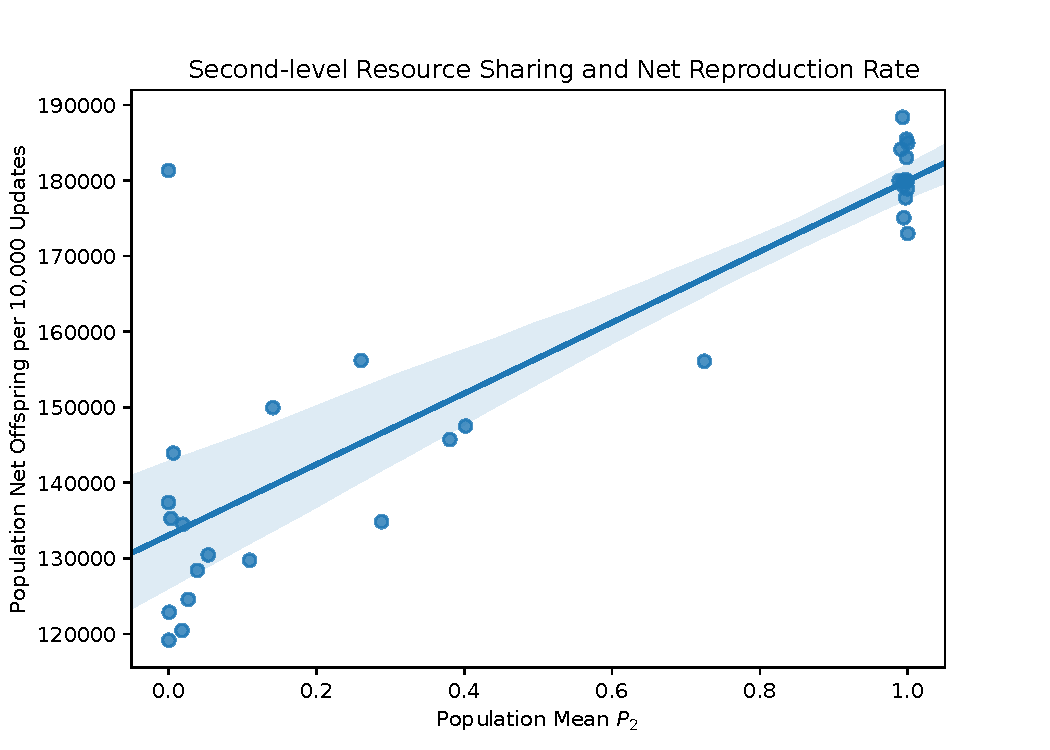
\includegraphics[width=0.7\textwidth]{results/mean_res_pool2_vs_net_reproduction}
\caption{
Correlation plot of population mean $P_2$ (resource-caching strategy) and population net reproduction rate.
A bootstrapped 95\% confidence interval for the fit is shaded.
}
\end{figure}

\end{frame}

\begin{frame}{Level-two Individuals' Apoptosis Response to Mutation}

\begin{figure}
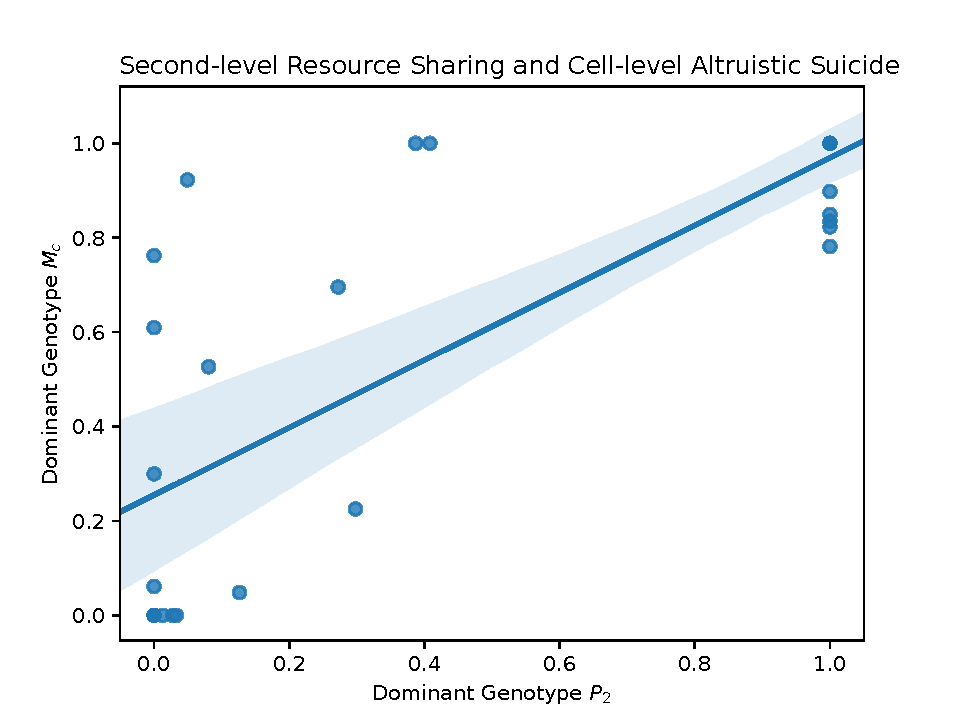
\includegraphics[width=0.7\textwidth]{results/champion_res_pool2_vs_champion_damage_suicide0}
\caption{
Correlation plot of dominant genotype $P_2$ (resource-caching strategy) and dominant genotype $M_{c}$ (apoptosis response to mutation).
A bootstrapped 95\% confidence interval for the fit is shaded.
}
\end{figure}

\end{frame}
